\section[Lehramtsstudium für Gymnasien \& Gesamtschulen (2-Fach-Bachelor)]{Lehramtsstudium für Gymnasien und Gesamtschulen (2-Fach-Bachelor)}
\begin{multicols*}{2}
Nachdem ihr es euch hoffentlich gut überlegt habt, Lehrerinnen und Lehrer zu werden, will ich euch an dieser Stelle in Münster begrüßen.
Was sich jetzt vielleicht abschreckend anhört, ist nicht ganz so gemeint.
Ich selber habe nun das 12.~Semester hinter mir und bin damit schon fast am Ende meines Studiums angelangt und bis jetzt mit meiner Entscheidung zufrieden.
Besonders nach dem Praktikum in der Schule weiß ich für mich, dass ich den richtigen Weg gewählt habe.

Aber eigentlich will ich hier nichts über mich erzählen, sondern euch in groben Zügen erklären, was so auf euch zukommt.
Es ist nicht lange her, da haben die sich ganz weit oben etwas Neues überlegt und so haben wir schon seit dem Wintersemester~2005/2006 Studenten an der Uni, die nicht mehr einfach Lehramt studieren, sondern den Abschluss Bachelor und anschließend den Master anstreben.
Dadurch habt ihr etwas mehr Glück, dass die ersten Probleme durch eure direkten Vorgänger (mich zum Beispiel ;-) ) schon aufgezeigt wurden und darauf reagiert wurde.
Was ihr im Laufe des Studiums alles in Physik machen müsst, das will ich hier genauer beschreiben.
Das Lehramtsstudium in Münster ist in mehrere Teile gegliedert.
Neben dem Fach Physik und einem weiteren Unterrichtsfach eurer Wahl (häufig ist das Mathematik, weswegen die Stundenpläne aufeinander abgestimmt werden) müsst ihr Bildungswissenschaften studieren.

\begin{center}
	\includegraphics[width=\columnwidth, height=0.2\textheight]{private/res/comics/calvin_schreibtisch.pdf}
\end{center}

\subsection{Was sind Module?}
In eurem Studium werden Vorlesungen, Übungen und Seminare in Modulen zusammengefasst und direkt im Anschluss in der Regel in einer Modulabschlussprüfung geprüft.
Alle Modulabschlussprüfungen gehen in eure Endnote ein -- mit der Ausnahme, dass bei den ersten drei Physik-Klausuren die mit der schlechtesten Note "gestrichen" wird (bestehen müsst ihr aber alle).
Das bedeutet für euch: Es reicht nicht einfach nur zu bestehen, sondern man muss schon von Anfang an versuchen, die besten Noten zu erreichen, damit die Endnote auch gut wird.
Das ist bei Klausuren aber nicht immer einfach.
Aber lasst euch davon nicht zu sehr stressen, schließlich sind Noten nicht alles.
Durch die Tatsache, dass die Modulabschlussprüfungen in die Bachelor-Note mit eingehen, ist es leider auch bedingt, dass jede Prüfung nicht beliebig oft gemacht werden darf.
In Physik~I--III habt ihr vier Versuche, in den anderen Prüfungen drei.
Wer sie nach diesen drei bzw.\ vier Versuchen nicht geschafft hat, kann sein Studium leider nicht fortsetzen.

\subsection{Die Grundmodule}
In den ersten drei Semestern belegt ihr die Module, welche die Grundlage für das Physikstudium bilden.
Diese Grundmodule sind die Module "Physik~I" (Dynamik der Teilchen und Teilchensysteme), "Physik~II" (Thermodynamik und Elektromagnetismus) und "Physik~III" (Wellen und Quanten).
Das Modul des ersten Semesters (Physik~I) ist für euch genauso wie für Studenten, die den 1-Fach-Bachelor machen.
Neuerdings bestehen die Module Physik~II und III nicht mehr jeweils nur aus den Vorlesungen des integrierten Kurses (wo jeweils ein Experimental-Professor und ein Theorie-Professor ihren Teil lesen) und den Übungen, sondern es gibt zusätzliche "Theoretische Ergänzungen".
Diese braucht ihr aber (anders als die 1-Fach-Bachelor) nicht zu besuchen.
In den Übungen bekommt ihr Aufgaben zu der Vorlesung und müsst diese rechnen.

Ihr habt damit nur Physik~I komplett gemeinsam mit den 1-Fach-Bachelor-Studenten -- es ist damit also nicht möglich, nach dem zweiten Semester ggf.\ ohne Zeitverlust in den 1-Fach-Bachelor zu wechseln, falls ihr nicht die theoretischen Ergänzungen belegt habt.
Solltet ihr also nach dem ersten Semester unsicher sein, ob ihr vielleicht wechseln wollt, wäre das ein Gedanke wert.
Dazu kommt noch das Modul "Experimentelle Übungen" im 3.\ und 4.~Semester, für das ihr etwa alle zwei Wochen einen Nachmittag in kleinen "Laboratorien" steht und einige Versuche durchführt.
Die Benotung der Module Physik~I--III erfolgt durch jeweils eine dreistündige Klausur, während es bei den Experimentellen Übungen Noten für jeden Versuch gibt (die jedoch nicht in die Endnote eingehen).

\subsection{Weitere Module}
Nach diesen drei Semestern habt ihr weitere Module aus verschiedenen Bereichen, die auf den Grundmodulen aufbauen.
Im 4.~Semester ist dieses das Modul "Atom- und Quantenphysik" (inoffiziell auch "Physik~IV" genannt), das aus den zwei Vorlesungen "Einführung in die Quantenmechanik" (Theorie) und "Atom- und Molekülphysik" (Experiment) besteht, zu denen es eine passende Übung gibt.
Hier habt ihr (anders als Studenten im 1-Fach-Bachelor) das erste Mal eine mündliche Prüfung von 30--45~Minuten.

Ab dem 5.~Semester könnt ihr im Modul "Anwendungen der Physik" die Vorlesung und Übungen zur Angewandten Physik und das Computerpraktikum besuchen, die mit einer mündlichen Modulabschlussprüfung abschließen.
Wann ihr diese mündliche Prüfung macht, könnt ihr mit dem jeweiligen Prüfer absprechen.
Die nächste mündliche Prüfung solltet ihr zum Abschluss des Moduls "Struktur der Materie" nach dem 5.~Semester haben.
Dieses Modul beinhaltet die drei Vorlesungen "Physik der kondensierten Materie", "Kern- und Teilchenphysik" und "Astrophysik und Kosmologie" sowie zwei Übungen zu der Vorlesung kondensierte Materie und zur Kern- und Teilchenphysik.
Dazu gehört auch noch ein frei wählbares Seminar aus diesem Bereich der Physik, in dem ihr einen Vortrag halten müsst.

Am Ende könnt ihr euch aussuchen, ob ihr eure Bachelorarbeit im Fach Physik oder in eurem zweiten Fach schreiben wollt.
In Physik müsst ihr aber auch noch einen halbstündigen Abschlussvortag über eure Arbeit halten.
Der sollte aber eigentlich keinen davon abhalten, da es eigentlich einfach ist, über seine Arbeit zu berichten, wenn man sich damit mehrere Wochen beschäftigt hat.

Es ist ratsam, mit der Bachelorarbeit schon in der vorlesungsfreien Zeit zwischen dem fünften und sechsten Semester anzufangen, weil es sonst wegen der Bearbeitungs- und Korrekturzeiten Probleme mit der rechtzeitigen Anmeldung für den Master geben könnte.
Die Prüfungsordnung findet ihr auf der \foreignlanguage{english}{Homepage} des Fachbereichs:
\begin{center}
	\url{https://www.uni-muenster.de/Physik}
\end{center}

\subsection{Bildungswissenschaften}
Die Bildungswissenschaften bestehen aus mehreren Modulen, die insgesamt \SI{20}{\LP} umfassen.
Zunächst absolviert ihr mit \SI{7}{\LP} das Modul "Einführung in Grundfragen von Erziehung und Bildung", in dem ihr eine Vorlesung mit Seminar besucht und das mit einer Klausur am Ende der Vorlesung abgeschlossen wird.
Auch gibt es das Eignungs- und Orientierungspraktikum mit \SI{6}{\LP}.
Hierbei besucht ihr ein Seminar zum Eignungs- und Orientierungspraktikum und macht ein fünfwöchiges Praktikum in einer Schule.
Als weiteres Praktikum absolviert ihr noch das Berufsfeldpraktikum mit \SI{7}{\LP}, in dem es um Berufsfelder geht, die nicht direkt mit der Aufgabe von Lehrern zusammenhängen.

\subsection{Schluss}
Das sind erst einmal alle Informationen, die ihr zum Physikstudium bis zum Bachelor braucht.
Die Informationen für das Masterstudium könnt ihr, sobald ihr soweit seid, durch die Fachschaft erfahren.
Trotz der Lektüre dieses Textes möchte ich euch die Informationsveranstaltung speziell für Zwei-Fach-Bachelor-Studenten in der Ersti-Woche ans Herz legen.
Dort habt ihr auch die Möglichkeit, direkt Fragen dazu zu stellen.
Ihr könnt aber auch jederzeit für die verschiedenen Fächer in den Fachschaften vorbei schauen; da ist meistens jemand, der euch weiterhelfen kann.
Natürlich gibt es auch noch die Beratung durch die Professoren oder die Zentrale Studienberatung~(ZSB).
Wer das wann und wo tut, erfahrt ihr u.\,a.\ auch in den Fachschaften.
Als letztes wünsche ich euch noch eine tolle Ersti-Woche (wahrscheinlich sehen wir uns), einen guten Start ins Studium, viel Glück beim "Leute kennenlernen" und -- vor allem -- viel Spaß in Münster.

\fibelsig{Bernd}

\begin{center}
	\fibelimgtext{
		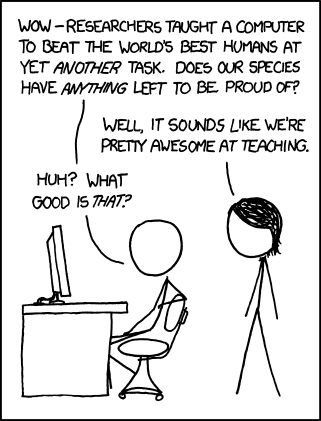
\includegraphics[width=\columnwidth, height=0.23\textheight]{res/xkcd/894_progeny.png}
	}{\url{https://xkcd.com/894}}
\end{center}
\end{multicols*}
